\section{Optimierung der Parameter des BDT-Algorithmus}
Bei dem Boosted Decision Tree wurde der AMS schlechter wenn Variablen entfernt wurden, daher wurde der volle Satz an Variablen verwendet. Um die optimalen Parameter für den BDT zu finden, haben wir für die Parameter
\begin{itemize}
	\item NTrees
	\item NEventsMin
	\item Shrinkage
	\item nCuts
	\item MaxDepth
\end{itemize} 
sinnvolle Bereiche festgelegt und wollten in diesem Parameterraum den besten AMS finden. Da die Laufzeit des Trainings für jeden Punkt im Parameterraum in der Größenordnung von Minuten liegt und wir 5 Parameter haben, lassen sich herkömmliche Optimierungsalgorithmen nicht sinnvoll anwenden.\\
Um einen Überblick zu erhalten ob es gewisse Bereiche gibt in denen der AMS generell besser ist, haben wir sehr oft (1389 mal) zufällige Parameter gewählt und den AMS dazu gespeichert. Wenn ein neuer Bestwert erreicht wurde, wurden die kontinuierlichen Parameter NEventsMin und Shrinkage Gaußverteilt um die zugehörigen Werte erzeugt.\\
Wie in den Abbildungen \ref{fig:AMS-distribution-plots} (a)-(e) zu erkennen ist, gibt es für einzelne Parameter kaum einen optimalen Wert. Aus diesem Grund haben wir uns für die Parameter entschieden mit denen wir den besten AMS-Wert erreicht hatten. Dies war der Fall bei
\begin{itemize}
	\item NTrees = 167
	\item NEventsMin = 7.28244760204
	\item Shrinkage = 0.0530833026321
	\item nCuts = 275
	\item MaxDepth  = 9  ,
\end{itemize} 
was auf den Trainingsdaten zu einem AMS-Wert von $0{,}773$ führte.

\begin{figure}[!t]
  \begin{tabular}[b]{cc}
	  \begin{subfigure}[b]{0.5\linewidth}
	   	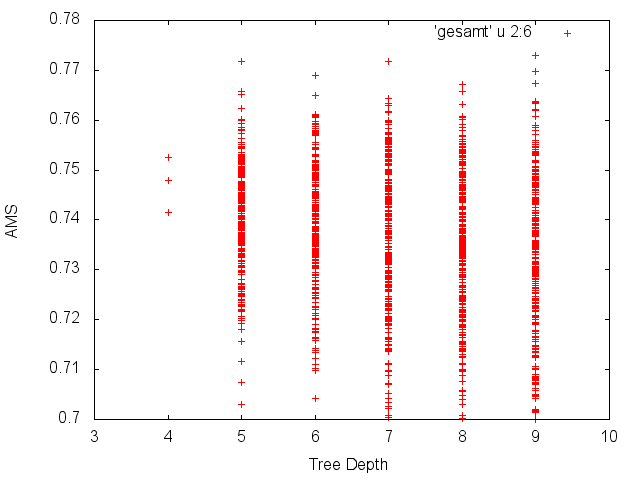
\includegraphics[width=\linewidth]{sections/parameter_optimization_bdt/Depth.png}
 		\caption[]{}
		\label{fig:bdt_Depth}
  	  \end{subfigure} &
  	  \begin{subfigure}[b]{0.5\linewidth}
  	  	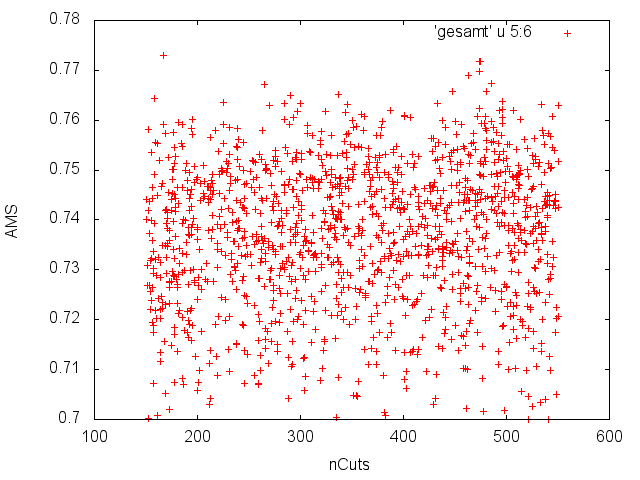
\includegraphics[width=\linewidth]{sections/parameter_optimization_bdt/nCuts.png}
 		\caption[]{}
		\label{fig:bdt_nCuts}
  	  \end{subfigure} \\
  	  
  	  \begin{subfigure}[b]{0.5\linewidth}
	   	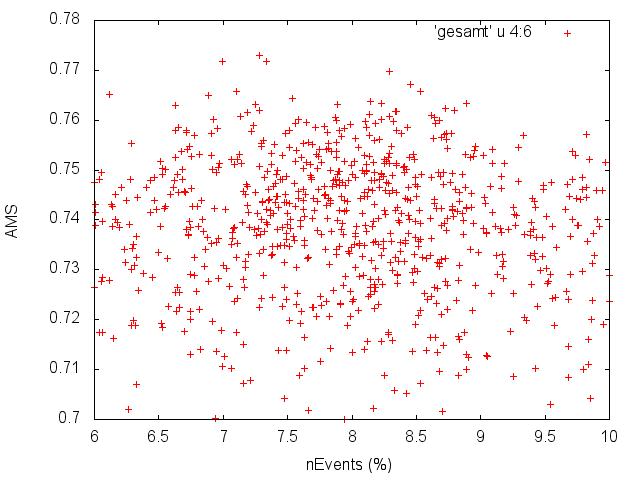
\includegraphics[width=\linewidth]{sections/parameter_optimization_bdt/nEvents.png}
 		\caption[]{}
		\label{fig:bdt_nEvents}
  	  \end{subfigure} &
  	  \begin{subfigure}[b]{0.5\linewidth}
  	  	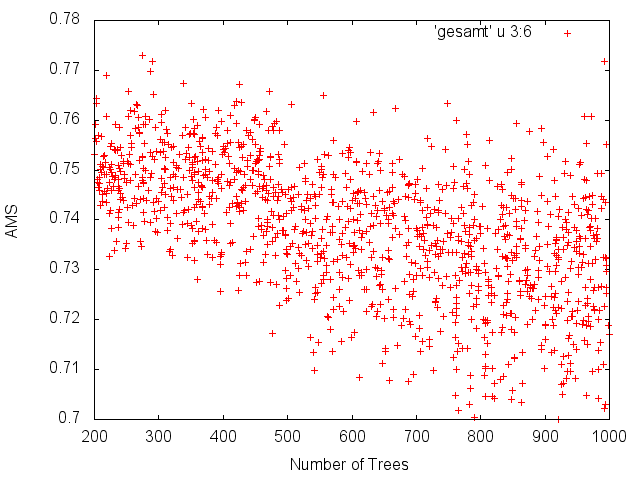
\includegraphics[width=\linewidth]{sections/parameter_optimization_bdt/Nt.png}
 		\caption[]{}
		\label{fig:bdt_Nt}
  	  \end{subfigure} \\
  	  
  	  \begin{subfigure}[b]{0.5\linewidth}
	   	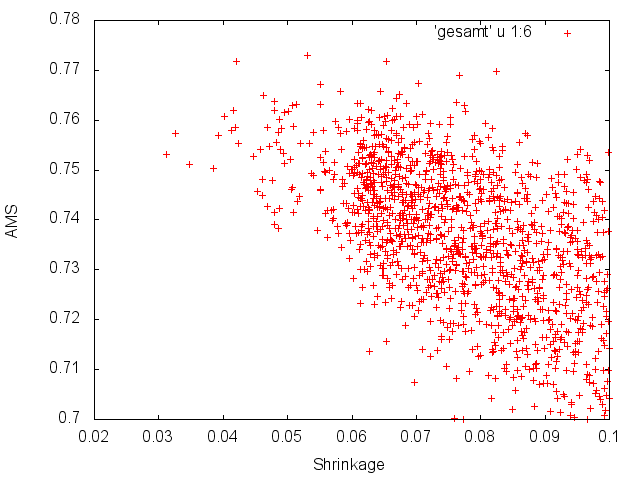
\includegraphics[width=\linewidth]{sections/parameter_optimization_bdt/Shrinkage.png}
 		\caption[]{}
		\label{fig:bdt_Shrinkage}
  	  \end{subfigure} &
  \end{tabular}
  \caption[]{AMS-Werte für die Parameter des Boosted Decision Tree als Scatter-Plots. Jeder Punkt entspricht einem Training}
  \label{fig:AMS-distribution-plots}
\end{figure}